
                \begin{figure}
                    \centering
                    \begin{tikzpicture}
                        \pgfplotsset{%
                            width=1\textwidth,
                            height=0.4\textheight
                        }
                        \begin{axis}[
                            xlabel={Start temperature},
                            ylabel={Average dynamic energy (watt)},
                            ymin=0,ymax=100,
                        ]
                        
                            \addplot [mark=none, densely dashed, red]  coordinates {
                            (35, 28.5570634918819)(40, 28.586306329601797)(45, 28.681706876409773)
                            };
                            \addlegendentry{workstation - IntelPowerGadget}
                            
                            \addplot [mark=none, densely dashed, blue]  coordinates {
                            (35, 30.614228060098657)(40, 28.488456665018205)(45, 28.582603357773348)(50, 28.60686955388757)
                            };
                            \addlegendentry{workstation - HardwareMonitor}
                            
                        \end{axis}
                    \end{tikzpicture} 
                \caption{A graph illustrating the energy consumption of Cores for test case Fasta with regards to the temperature of the DUT (without outliers)} \label{fig:Fasta_Cores_temperature_exp2}
                \end{figure}
                